\chapter{Evaluation}

This section presents a comprehensive evaluation of the proposed trading
mechanism, focusing on its performance, scalability, and overall effectiveness
in multi cluster environments. We employ a combination of synthetic and
real-world workloads to simulate various scenarios, alongside an array of rules
and policies to investigate beneficial strategies and the effectiveness of
different workload-strategy combinations.

However, the possible combinations of rules, policies and their respective
configurations is infinite. Our aim in this section is not to exhaust all
possibilities, but to explore the validity of the mechanism under different
constraints. This approach paves the way for users to conduct their experiments
on thier specific workloads to determine the strategy that best fits their
needs.  

All experiments are run on Cloudlab, a scientific infrastructure used by
academics for systems and cloud research \cite{duplyakin_design_2019}. We
utilize the following setups to to run the experiments. Each node in the setups
simulates one cluster, with the cluster, trader, and client running on the same
machine. 
% CITE CLOUDLAB NODES
\begin{enumerate}

  \item \textbf{Setup One:} 3 Cloudlab nodes c6525-100g running Linux
    Ubuntu 22.04 in the same Utah datacenter.

  \item \textbf{Setup Two:} 3 Cloudlab nodes of type m510, c220g1, c8220
    running on three distinct datacenters in Utah, Wisconsin, and Clemson.
\end{enumerate}

The setups simulate different scenarios where clusters can belong to one
organization or different organizations, and have varying network latency and
bandwidth.  

We derive our results by running a configuration of rules, policies, and
workloads twice, once with and once without the mechanism and compare the
performance difference.

Our methodology for running workloads is as follows: All participating clusters
have the same start and end time for receiving jobs from their respective
clients. After the clients stop sending jobs, the experiment is kept on until
the last job in the slowest cluster finish execution. 

\section{Experiment One}
\vspace{2em}
\begin{center}
  \fbox{\parbox{14cm}{
  
    \underline{Configuration:}
    \vspace{.3em}
    \begin{enumerate}
  
      \item \textbf{Setup:} \#1 with three cooperative clusters.
  
      \item \textbf{Workload:} Synthetic, all clusters are oversubscribed.
      
      \item \textbf{Rules:} Approve trades if average wait time is below 5
        seconds and both memory and core utilization below 0.8
      
      \item \textbf{Policies:} Initiate trades if utilization is above 0.8 or
        average wait time above 60 seconds.
  
    \end{enumerate}
  }}
\end{center}
We will first examine the scenario where all cooperative clusters have high
resource utilization for the entirety of the experiment duration.

%We aim by this experiment to showcase the overhead of the trading mechanism
%where it's likely not beneficial to participate.

\begin{figure}[H]
\centering
\begin{subfigure}{.5\textwidth}
  \centering
  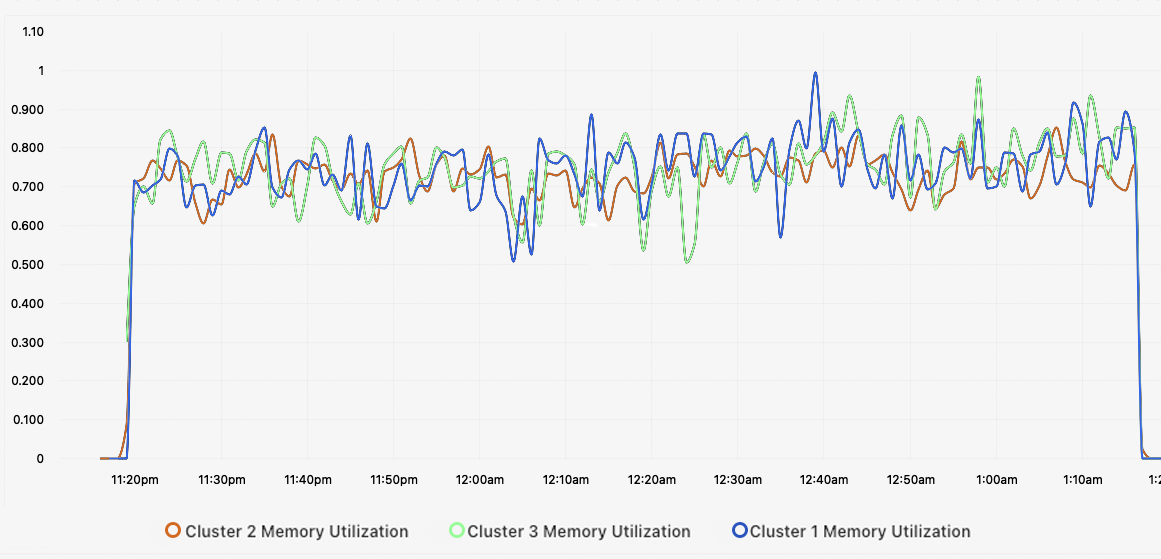
\includegraphics[width=.9\linewidth]{./figures/experiment-one/exp-one.png}
  \caption{cooperative clusters}
  \label{fig:exp1coop}
\end{subfigure}%
\begin{subfigure}{.5\textwidth}
  \centering
  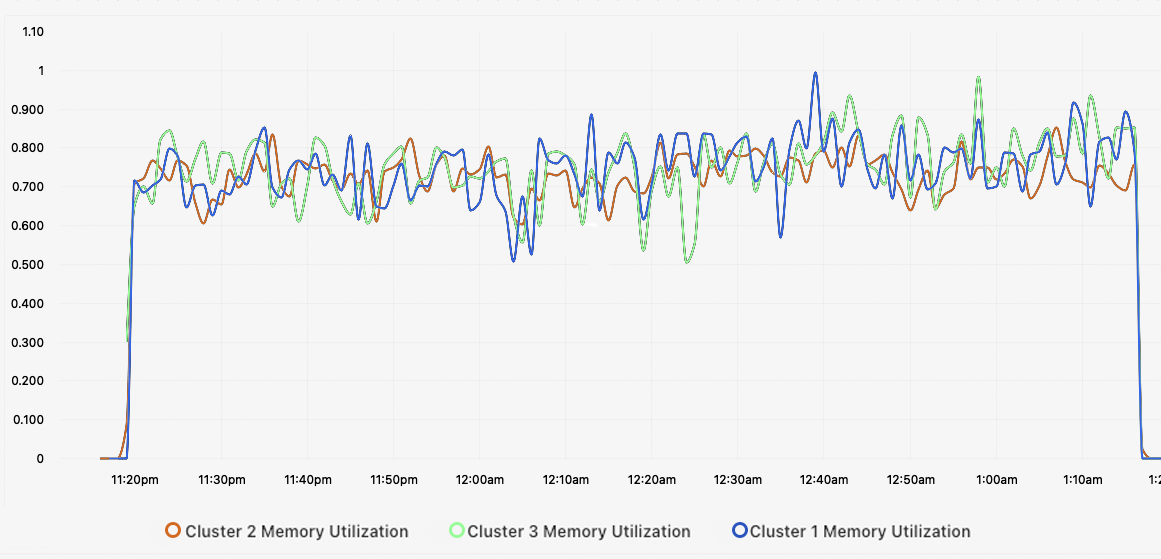
\includegraphics[width=.9\linewidth]{./figures/experiment-one/exp-one-control.png}
  \caption{control cluster}
  \label{fig:exp1control}
\end{subfigure}
\caption{Experiment 1, memory utilization.}
\label{fig:exp1memutil}
\end{figure}

Figure~\ref{fig:exp1memutil} presents the memory utilization of the cooperative
clusters in Figure~\ref{fig:exp1coop} and the same workload run on a cluster without
trading in Figure~\ref{fig:exp1control}.
% analysis
We can see that the control cluster have a slightly lower utilization averaging
at 70\% whereas cooperative clusters' memory utilization averaged at 75\%. This
5\% difference is due to cooperative clusters doing quick trades during short
downtime intervals, leading to an inefficient scheduling and coupled with
higher utilization. In this case, trading is discouraged or a higher buffer
between trades is preferred. We can draw the same conclusion for the difference
in core utilization with 65\% and 71\%. However, this led to a 5.45\% increase
in total time to finish all jobs as local resources were occationally lent
just before a spike in jobs, delaying the execution of the local ones. As this
phenomenon happened on all clusters, they all suffered decreased performance.
It's important to mention that a cluster can't evict external allocations once
the contract is approved, hence a trade can be expensive without proper
considerations.

We can see this effect play out in the number of jobs in the scheduler's queues.
\begin{figure}[H]
  \begin{center}
    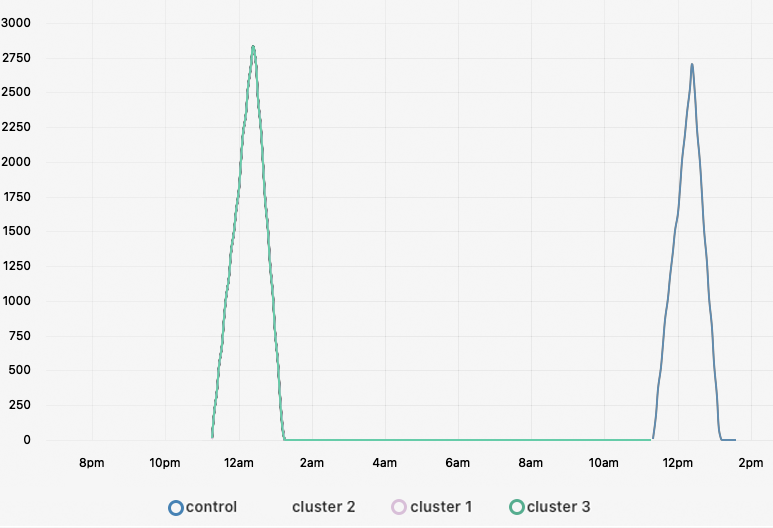
\includegraphics[width=0.5\textwidth]{./figures/experiment-one/jobs-in-queue.png}
  \end{center}
  \caption{Jobs in queue.}
  \label{fig:exp-1-jobs-in-queue}
\end{figure}

As seen in Figure~\ref{fig:exp-1-jobs-in-queue}, all participating
clusters incurred an increased number of jobs in the queue at the peak. Note
that the peak is created because of our workload methodology. The decreasing
part of the graph resembles the cool down time, or the time it takes to finish
scheduling all jobs after the client is done sending them. As all these clusters
are oversubscribed; jobs keep getting queued until the client is done 
sending. The total workload per cluster in this experiment was around 8000
jobs. 

\section{Experiment Two}
\vspace{2em}
\begin{center}
  \fbox{\parbox{14cm}{
  
    \underline{Configuration:}
    \vspace{.3em}
    \begin{enumerate}
  
      \item \textbf{Setup:} \#1 with three cooperative clusters.
  
      \item \textbf{Workload:} Synthetic 
        \vspace{-.5em}
          \begin{enumerate}
            \item One underutilized. 
            \item One highly utilized. 
            \item One oversubscribed. 
          \end{enumerate} 
      
      \item \textbf{Rules:} Approve trades if average wait time is below 5
        seconds and both memory and core utilization below 0.8
      
      \item \textbf{Policies:} Initiate trades if utilization is above 0.8 or
        average wait time above 60 seconds.
  
    \end{enumerate}
  }}
\end{center}

In this experiment, we run trading on a similar rule and policy configuration
as experiment one but with varying workloads between clusters, detailed in the
configuration box above. 

\begin{figure}[H]
\centering
\begin{subfigure}{.5\textwidth}
  \centering
  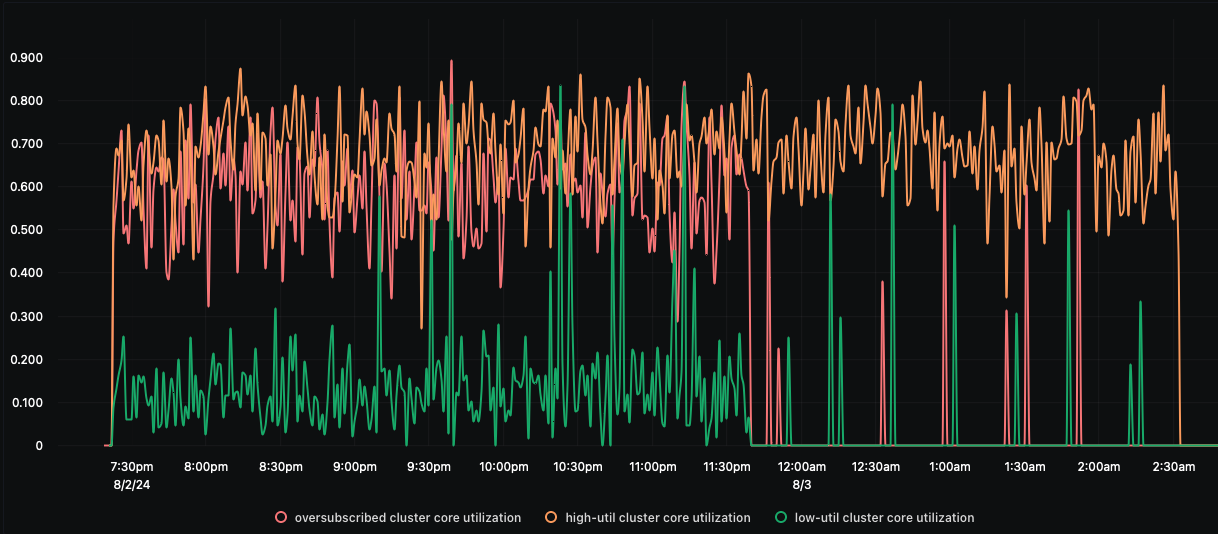
\includegraphics[width=.9\linewidth]{./figures/experiment-two/exp-two-coop.png}
  \caption{cooperative clusters}
  \label{fig:exp2coop}
\end{subfigure}%
\begin{subfigure}{.5\textwidth}
  \centering
  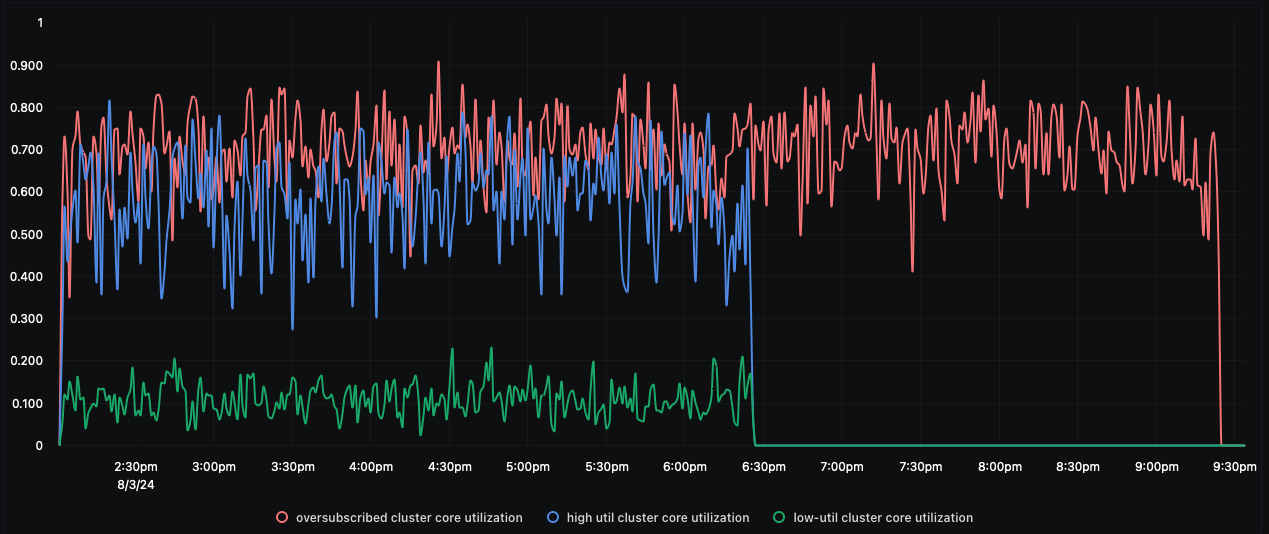
\includegraphics[width=.9\linewidth]{./figures/experiment-two/exp-two-control.png}
  \caption{control cluster}
  \label{fig:exp2control}
\end{subfigure}
\caption{Experiment 2, core utilization.}
\label{fig:exp2coreutil}
\end{figure}

Figure~\ref{fig:exp2coreutil} displays the core utilization of the cooperative
clusters in Figure~\ref{fig:exp2coop} and the same workload run on a cluster without
trading in Figure~\ref{fig:exp2control}.
% analysis
The first evident difference between the two graphs is the spikes seen on the
underutilized cluster and less apparent on the highly utilized. These
indicate the occurence of trades, benefiting the highly utilized 100
jobs/minute cluster. Trading did not negatively affect the performance of any
of the particpating clusters, and it decreased the total time to finish all jobs in
the environment by 5.8\%, from 7 hours and 28 minutes to 7 hours.

\section{Experiment Three}
\vspace{2em}
\begin{center}
  \fbox{\parbox{14cm}{
  
    \underline{Configuration:}
    \vspace{.3em}
    \begin{enumerate}
  
      \item \textbf{Setup:} \#1 with three cooperative clusters.

      \item \textbf{Workload:} Synthetic
          \vspace{-.5em}
          \begin{enumerate}
            \item Two highly utilized clusters
            \item One small cluster with varying utilization levels 
          \end{enumerate} 
      \item \textbf{Rules:} Approve trades if average wait time is below 5
        seconds and both memory and core utilization below 0.8
      
      \item \textbf{Policies:} Initiate trades if utilization is above 0.8 or
        average wait time above 60 seconds.
  
    \end{enumerate}
  }}
\end{center}

This experiment models a scenario with some similarity to the machine learning
training-inference workloads the Lyra system takes advantage of
\cite{li_lyra_2023}, albeit with some differences. There are two big highly
utilized clusters, and one small cluster experiencing low utilization in
addition to spikes. We kept the rules and policies similar to the previous
experiments for reference. Figure~\ref{fig:exp3memutil} shows the memory utilization of
these clusters. 

\begin{figure}[H]
\centering
\begin{subfigure}{.5\textwidth}
  \centering
  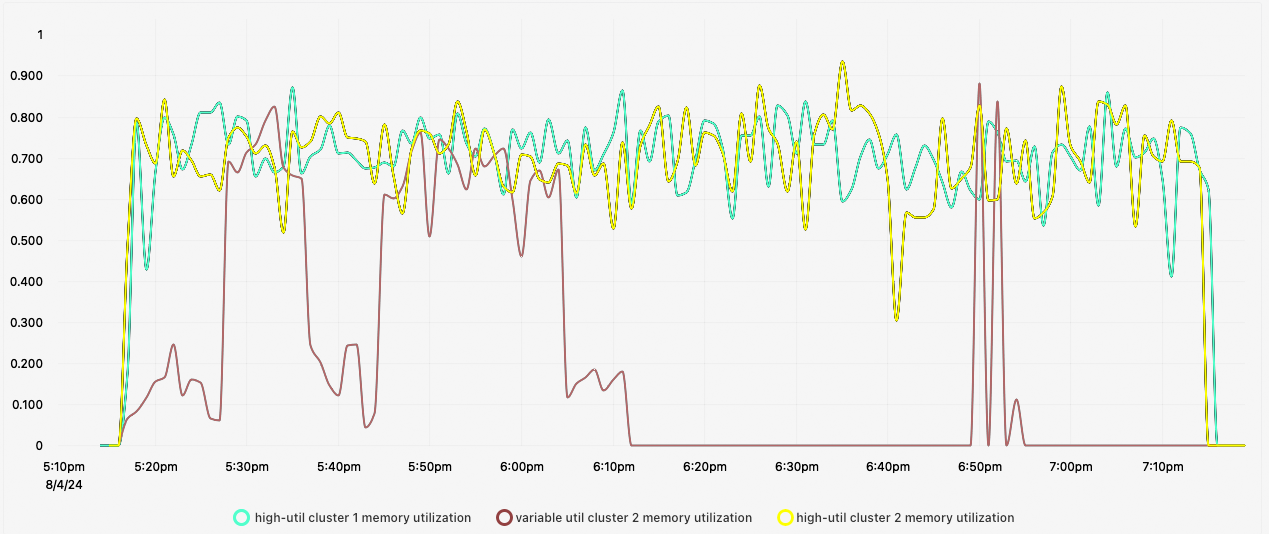
\includegraphics[width=.9\linewidth]{./figures/experiment-three/exp-three-coop.png}
  \caption{cooperative clusters}
  \label{fig:exp3coop}
\end{subfigure}%
\begin{subfigure}{.5\textwidth}
  \centering
  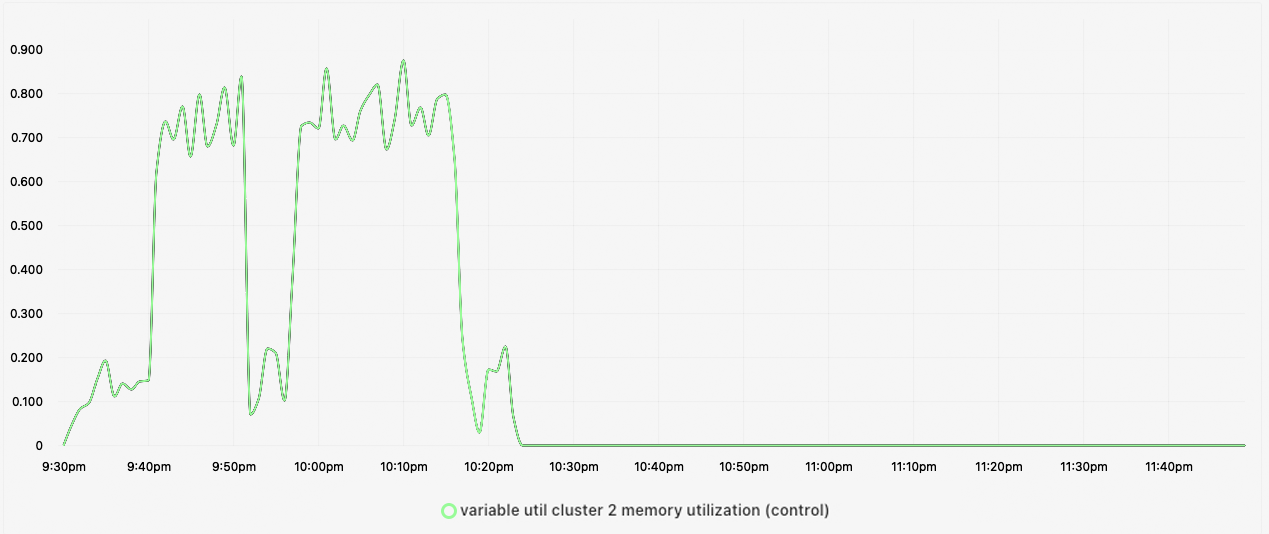
\includegraphics[width=.9\linewidth]{./figures/experiment-three/exp-three-control.png}
  \caption{control cluster}
  \label{fig:exp3control}
\end{subfigure}
\caption{Experiment 3, memory utilization.}
\label{fig:exp3memutil}
\end{figure}

The small cluster did not incur any degradation for loaning its resources, as
job completion time and total time to finish all jobs remained the same as shown
in Figure~\ref{fig:exp3memutil}. The highly utilized clusters were able to manage their workloads for most of the
experiment, with the small cluster experiencing only 15\% increase in
utilization. This led to a  4\% reduction in time to schedule all jobs in the
highly utilized clusters. 

\section{Experiment Four}
\vspace{2em}
\begin{center}
  \fbox{\parbox{14cm}{
  
    \underline{Configuration:}
    \vspace{.3em}
    \begin{enumerate}
  
      \item \textbf{Setup:} \#1 with two opportunistic clusters.

      \item \textbf{Workload:} Synthetic
          \vspace{-.5em}
          \begin{enumerate}
            \item One highly utilized cluster
            \item One underutilized cluster
          \end{enumerate} 
      \item \textbf{Rules:} Approve trades if average wait time is below 5
        seconds and both memory and core utilization below 0.8 AND incentive 
        provided is higher than current cost of operation.
      
      \item \textbf{Policies:} Initiate trades if utilization is above 0.8 or
        average wait time above 5 seconds AND there's a budget for a trade.
  
    \end{enumerate}
  }}
\end{center}

In this experiment, we study the effects of having two opportunistic clusters
in the system. We assume that both clusters' cost for resource is the same,
which is the price of Microsoft Azure's general purpose instance
\cite{azure_pricing}. This price would be the maximum any cluster would pay for
a resource, as an alternate is clearly available. The cluster's value of a
resource varies in relation to, and is directly proportional, to its
utilization.

\begin{figure}[H]
\centering
\begin{subfigure}{.5\textwidth}
  \centering
  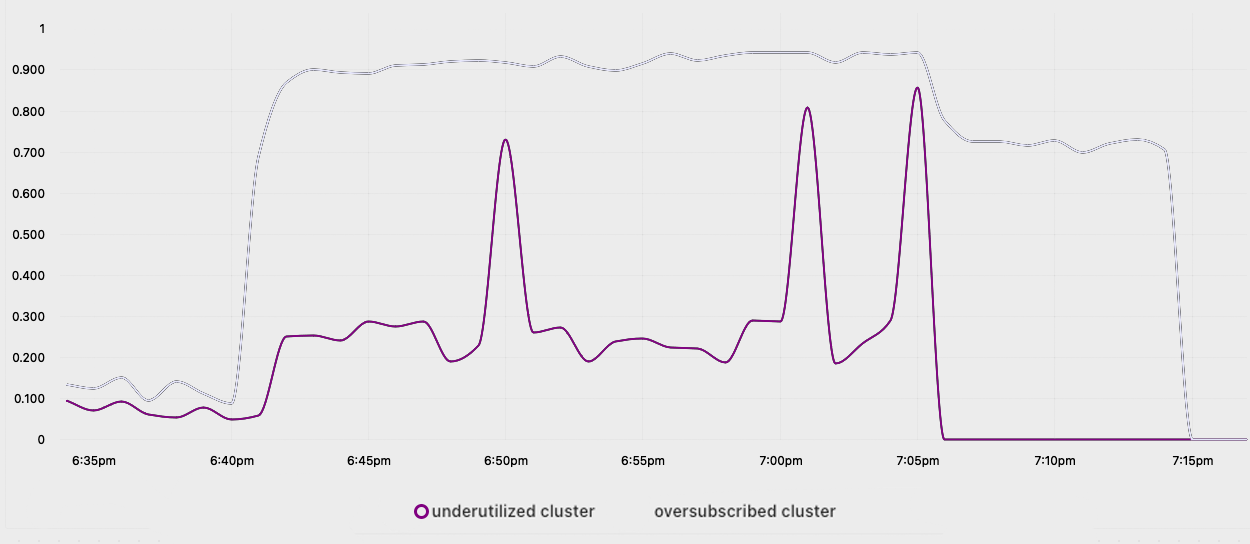
\includegraphics[width=.9\linewidth]{./figures/experiment-four/exp4-incentives-2.png}
  \caption{opportunistic clusters}
  \label{fig:exp4oop}
\end{subfigure}%
\begin{subfigure}{.5\textwidth}
  \centering
  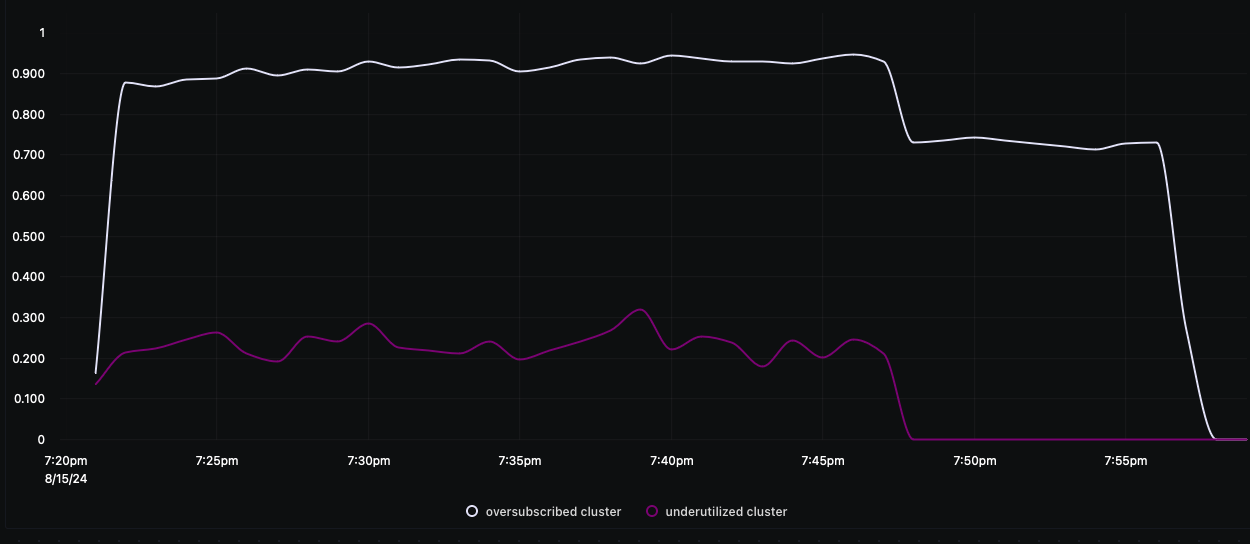
\includegraphics[width=.9\linewidth]{./figures/experiment-four/exp4-incentives-control-2.png}
  \caption{control clusters}
  \label{fig:exp4control}
\end{subfigure}
\caption{Experiment 4, memory utilization.}
\label{fig:exp4memutil}
\end{figure}

As the Figure~\ref{fig:exp4oop} shows, the underutilized cluster experienced spikes in
utilization caused by successful trades, which led to a 12\% increase in
utilization. The trades also reduced the cluster's cost by 3\%. The highly
utilized cluster witnessed an 8\% reduction in total job completion time (TJCT)
while also reducing the cost by 3\%.

\section{Experiment Five}
\vspace{2em}
\begin{center}
  \fbox{\parbox{14cm}{
  
    \underline{Configuration:}
    \vspace{.3em}
    \begin{enumerate}
  
      \item \textbf{Setup:} \#2 with two cooperative clusters.

      \item \textbf{Workload:} Production
          \vspace{-.5em}
          \begin{enumerate}
            \item small: 1.3k machine cluster
            \item large: 4k machine cluster
          \end{enumerate} 
      \item \textbf{Rules:} Approve trades if average wait time is below 5
        seconds and both memory and core utilization below 0.8.
      
      \item \textbf{Policies:} Initiate trades if utilization is above 0.8 or
        average wait time above 5 seconds.
  
    \end{enumerate}
  }}
\end{center}

This experiment studies the effects of introducing cooperative trading to two
Alibaba clusters. Both clusters run both long running applications and short
spanned jobs. The small cluster trace was recorded in 2017 while the large
cluster trace was recorded in 2018. Although large cluster trace spans for 8
days, we're bound by the small cluster's period of 12 hours, so a random 12
hour period was picked from the large cluster with the same starting time. 

Figures \ref{fig:exp5memutil} and \ref{fig:exp5coreutil} represent the reported core and memory utilization from
the experiment.

\begin{figure}[H]
\centering
\begin{subfigure}{.5\textwidth}
  \centering
  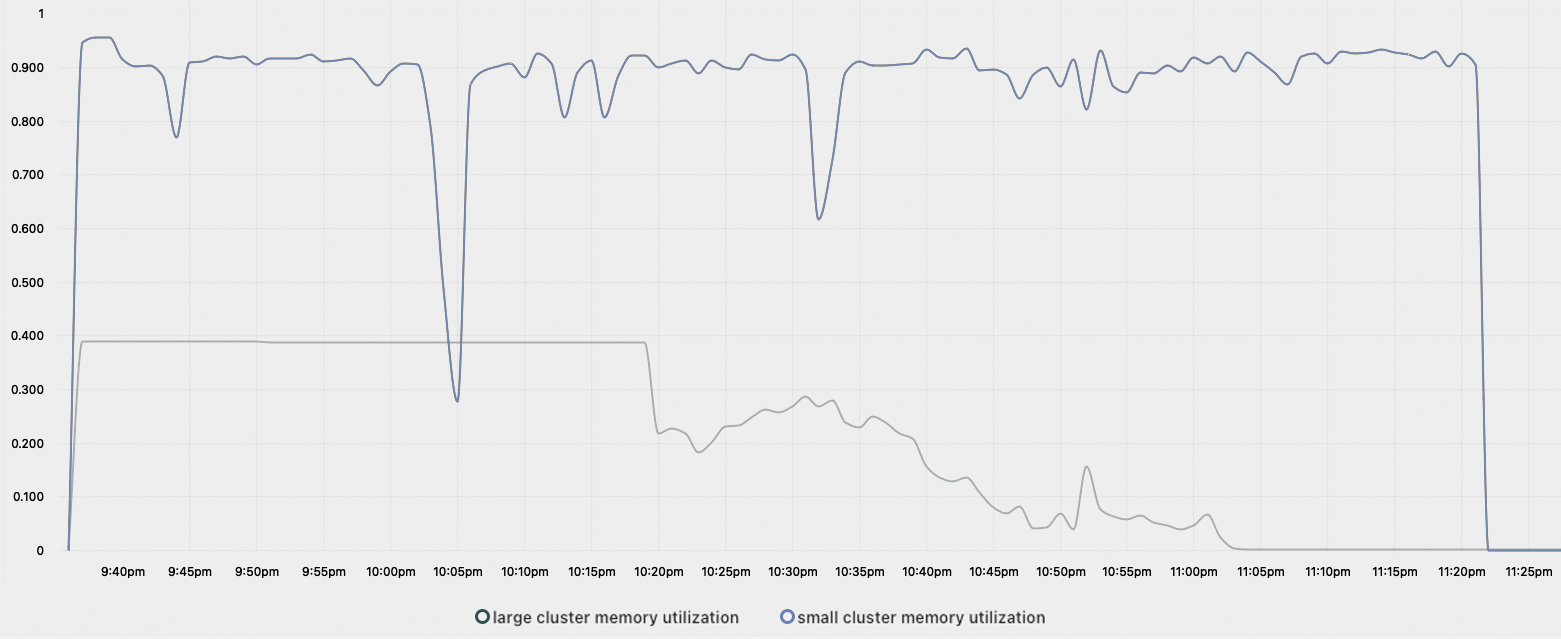
\includegraphics[width=.9\linewidth]{./figures/experiment-five/alibaba-mem-coop.png}
  \caption{cooperative clusters memory utilization}
  \label{fig:exp5coopmem}
\end{subfigure}%
\begin{subfigure}{.5\textwidth}
  \centering
  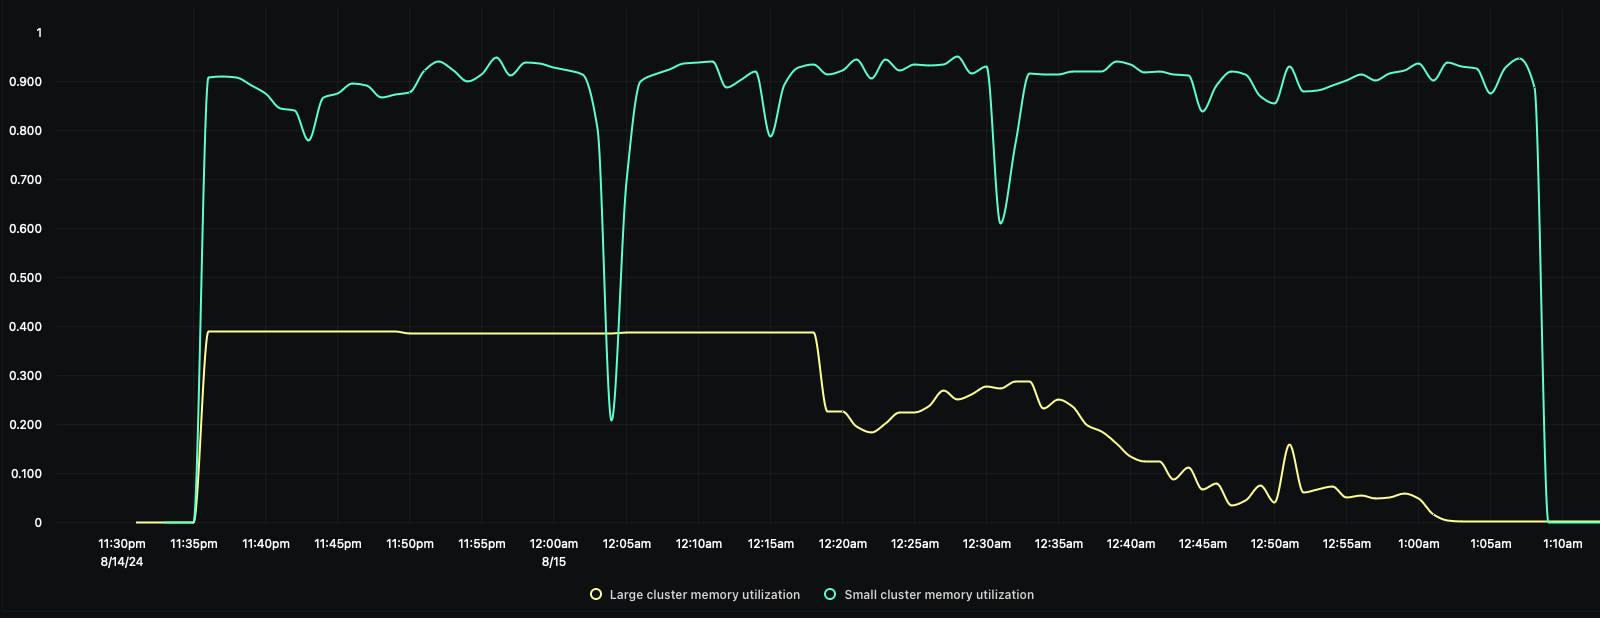
\includegraphics[width=.9\linewidth]{./figures/experiment-five/alibaba-mem-control.png}
  \caption{control clusters memory utilization}
  \label{fig:exp5controlmem}
\end{subfigure}
\caption{Experiment 5, memory utilization.}
\label{fig:exp5memutil}
\end{figure}

The memory utilization of the small cluster was nearing 100\% for the entirety
of the experiment, whereas the large cluster didn't go above 40\%. We can't see
much of a difference between the two graphs meaning that just a small amount of
tradering was accomplished. This is due to the core utilization, explained
below.

\begin{figure}[H]
\centering
\begin{subfigure}{.5\textwidth}
  \centering
  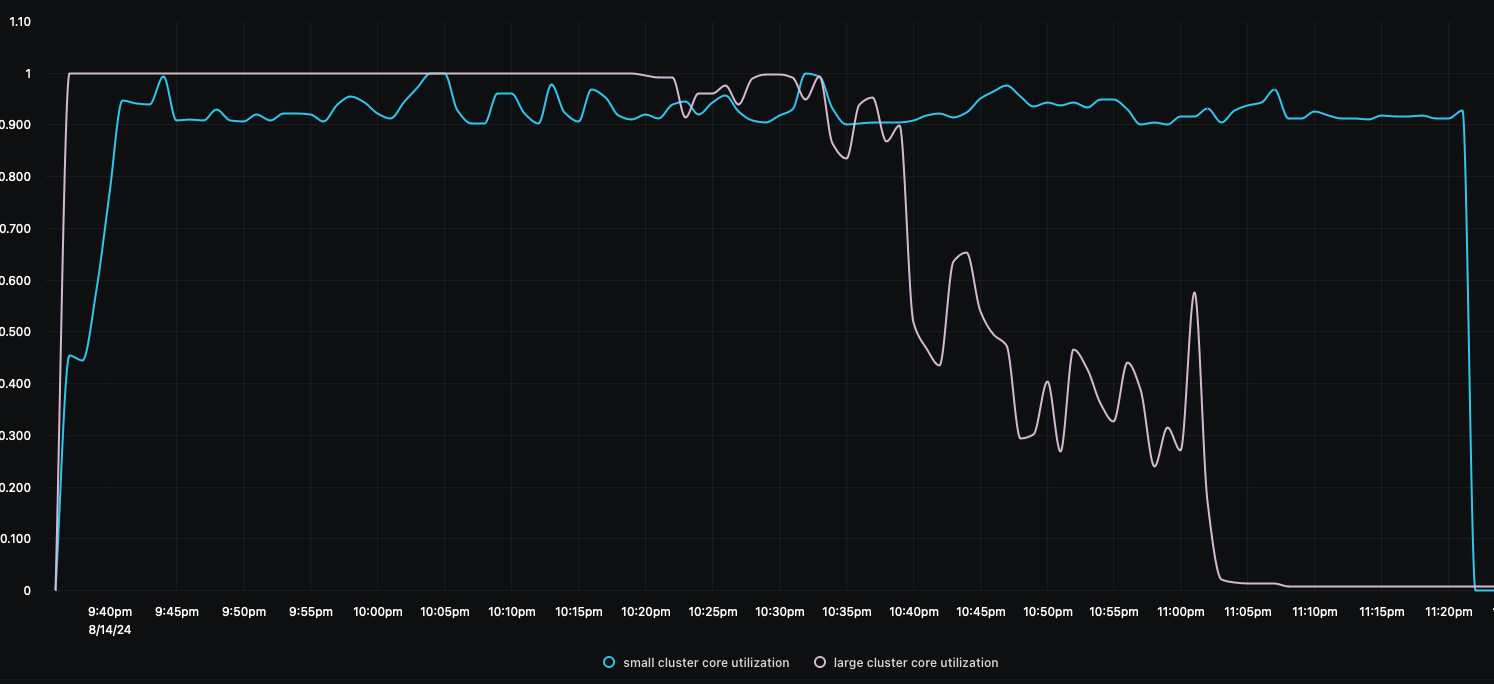
\includegraphics[width=.9\linewidth]{./figures/experiment-five/alibaba-core-coop.png}
  \caption{cooperative clusters core utilization}
  \label{fig:exp5coopcore}
\end{subfigure}%
\begin{subfigure}{.5\textwidth}
  \centering
  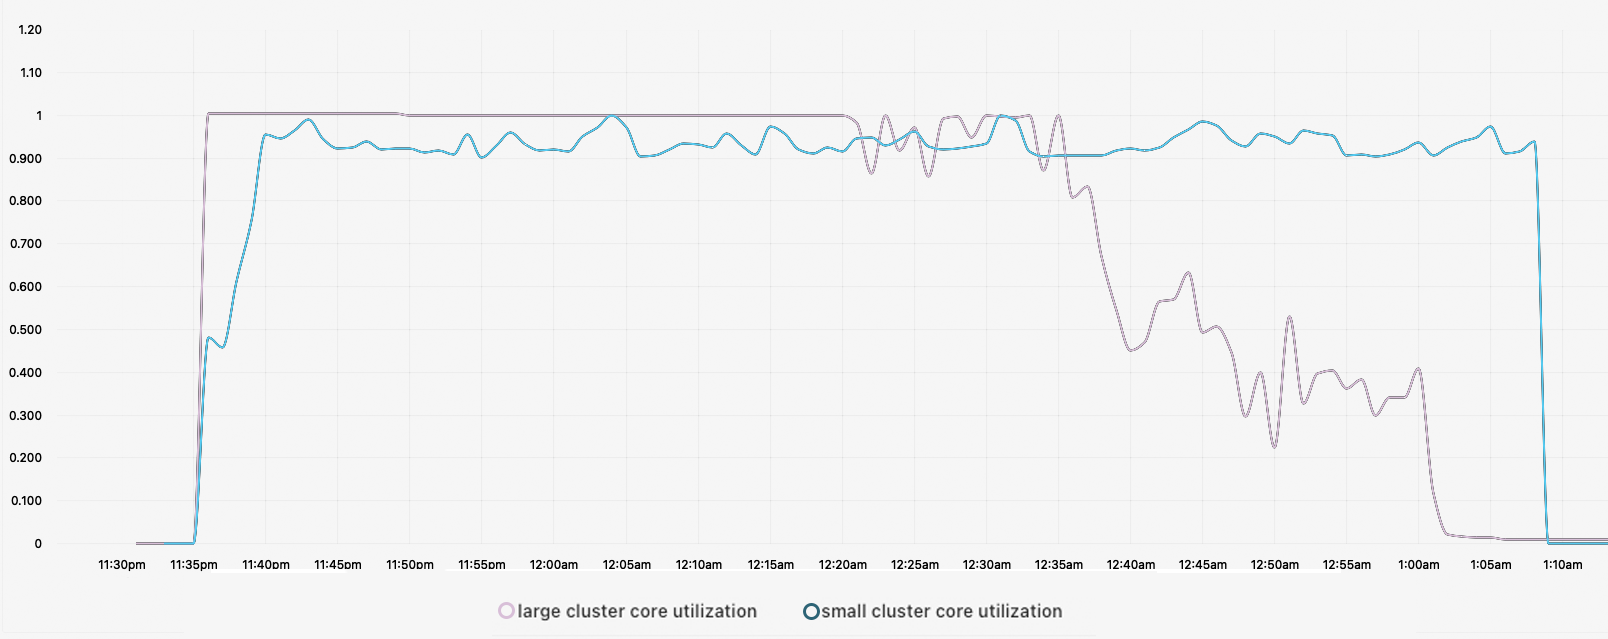
\includegraphics[width=.9\linewidth]{./figures/experiment-five/alibaba-core-control.png}
  \caption{control clusters core utilization}
  \label{fig:exp5controlcore}
\end{subfigure}
\caption{Experiment 5, core utilization.}
\label{fig:exp5coreutil}
\end{figure}

We can see that the core utilization in the small cluster was at 90\% for all
the experiment duration. On the other hand, the large cluster was fully
utilized up until the very end. Trading only occurred during this duration, and
led to a 2\% increase in the large cluster's utilization and a 1\% reduction in
the TJCT.

\section{Experiment Six}
\vspace{2em}
\begin{center}
  \fbox{\parbox{14cm}{
  
    \underline{Configuration:}
    \vspace{.3em}
    \begin{enumerate}
  
      \item \textbf{Setup:} \#1 with two cooperative clusters.

      \item \textbf{Workload:} Synthetic 
          \vspace{-.5em}
          \begin{enumerate}
            \item One over-utilized cluster
            \item One diurnally-utilized cluster
          \end{enumerate} 
      \item \textbf{Rules:} Approve trades if average wait time is below 5
        seconds and both memory and core utilization below 0.8.
      
      \item \textbf{Policies:} Initiate trades if utilization is above 0.8 or
        average wait time above 5 seconds.
  
    \end{enumerate}
  }}
\end{center}

In this experiment, we replicate the setup present in the Lyra system
\cite{li_lyra_2023}, with the difference being that lending clusters are
restricted from evicting jobs already scheduled on their nodes. The training
cluster is over-subscribed to present the elastic nature of training workloads,
whereas the inference cluster follows a diurnal pattern resembling the clients'
inference usage. Both clusters are simulated with an equal size of 100 nodes.  

\begin{figure}[H]
\centering
\begin{subfigure}{.5\textwidth}
  \centering
  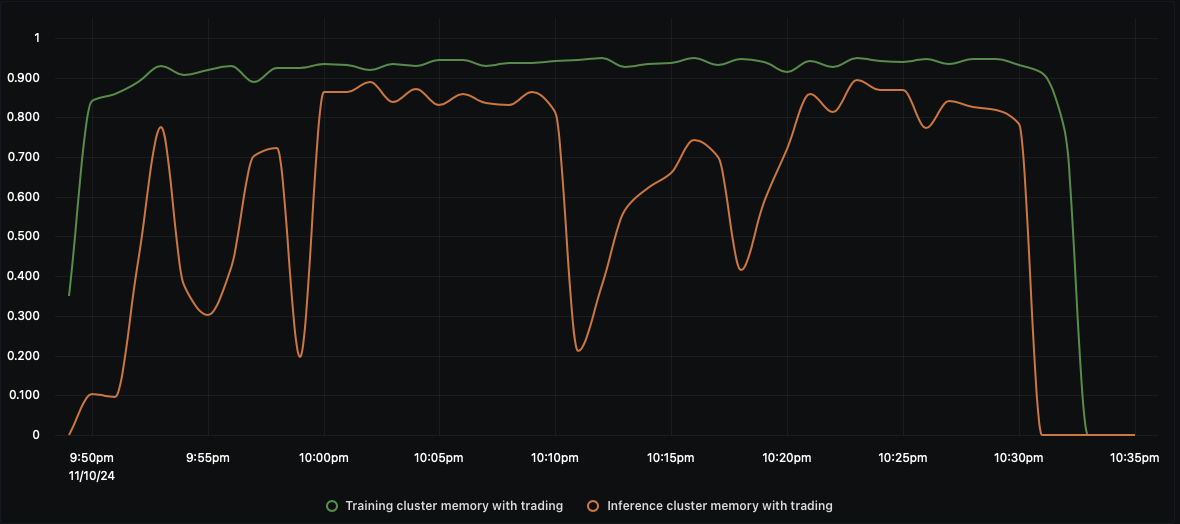
\includegraphics[width=.9\linewidth]{./figures/experiment-six/trading.png}
  \caption{cooperative clusters core utilization}
  \label{fig:exp6coop}
\end{subfigure}%
\begin{subfigure}{.5\textwidth}
  \centering
  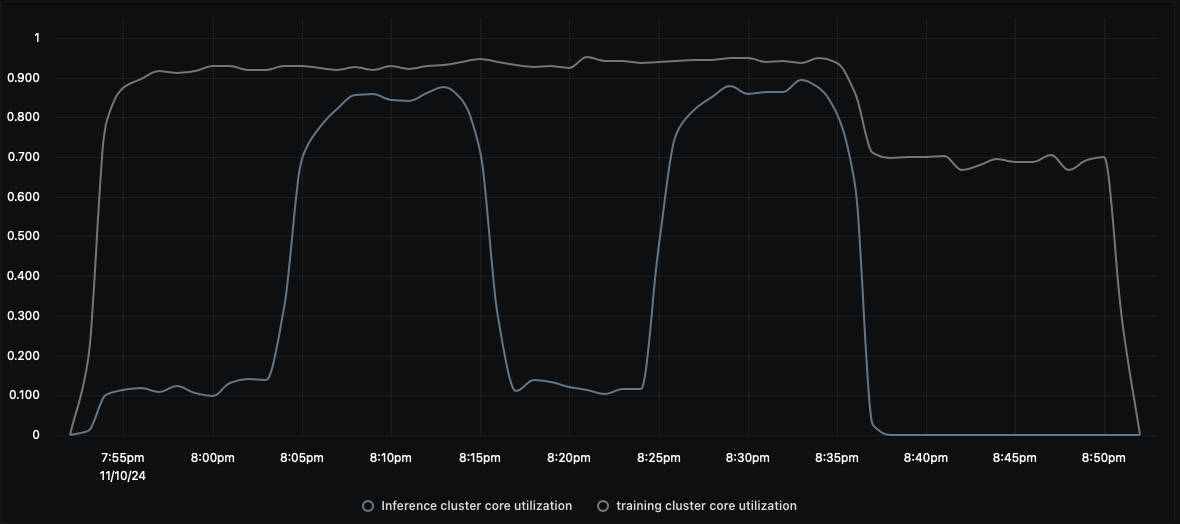
\includegraphics[width=.9\linewidth]{./figures/experiment-six/control.png}
  \caption{control clusters core utilization}
  \label{fig:exp6control}
\end{subfigure}
\caption{Experiment 6, core utilization.}
\label{fig:exp6coreutil}
\end{figure}

As illustrated in Figure~\ref{fig:exp6coop}, the inference cluster's resources
during downtime was efficiently utilized through trading compared to the
control scenario depicted in Figure~\ref{fig:exp6control}. This led to a six
fold increase in resource utilization in the inference cluster without
negatively impacting the traininig cluster. The optimized resource usage
contributed to 34\% increase in (TJCT). We can also notice that the graph in
the highly utilized` section of the diurnal pattern in Figure~\ref{fig:exp6coop} shows
more variability than Figure~\ref{fig:exp6coop} due to the restrictions on eviction.
